\section{Introduction}

Connectomics, the field of large-scale nanometer reconstruction of the wiring diagram of the brain, has created datasets petabytes in size (FIX). These datasets are too large for manual reconstruction. 



\begin{itemize}
	\item Connectomics background
	\item Problem Statement
	\item Summary of previous work (lite)
	\item Summary of our method
	\item Summary of contributions
\end{itemize}

\begin{figure}
	\centering
	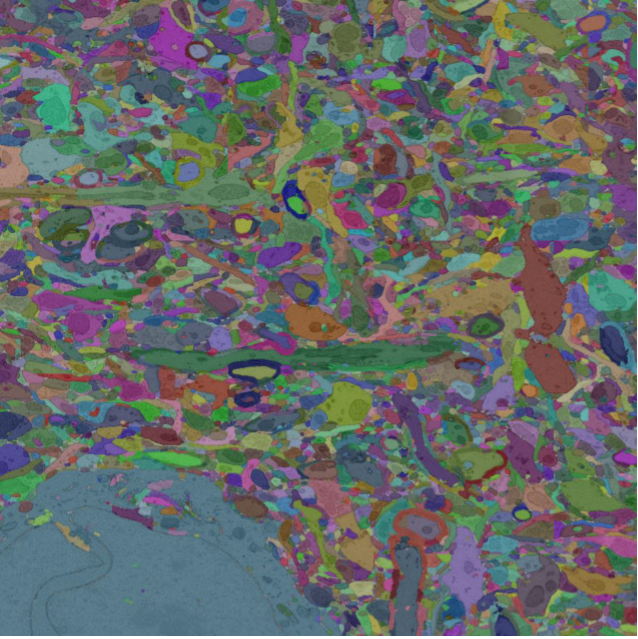
\includegraphics[width=0.42\linewidth]{./figures/intro-slice.png}
	\hspace{0.085\linewidth}
	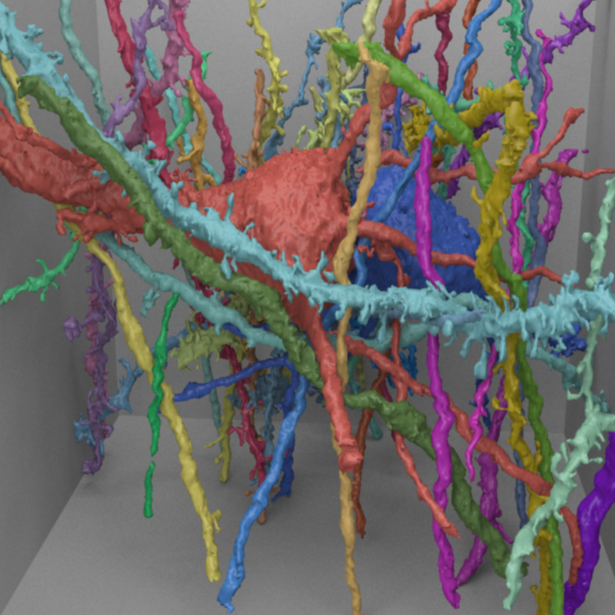
\includegraphics[width=0.42\linewidth]{./figures/intro-cube.png}
\end{figure}

The lowest-level frameworks in connectomics focus on per-pixel decisions using localized information. 
In addition, (write names) et al. use the multi-cut segmentation algorithm on the raw image data to produce segmentations.
Recently, significant research focuses on developing per-pixel affinity and boundary membrane predictions using 3D convolutional neural networks (CITE VD2D3D, U-NET).
Although these low-level algorithms have seen dramatic improvements in recent years, they do not fully leverage all available information.
Therefore, researchers began constructing algorithms that build another level of abstraction above the per-pixel level that trained random forest classifiers using shape features at the superpixel level (CITE GALA, NeuroProof).

Although these most recent advances produce impressive improvements on the original per-pixel algorithms, they do not fully integrate the full information provided by the datasets.
In this paper we provide a new framework which builds a new level of abstraction on top of the existing research. 
We construct a graphical representation from the outputs of the per-superpixel agglomeration strategies to further improve the merging results.
We focus on the shapes of the segments to make merge and split decisions. 
We provide three main contributions: using a skeleton representation of the 3D segments to predict merge locations, training a 3D convolutional neural network on the segment shapes to predict merging, and a new level of abstraction on the data that considers the data in a graphical form.